\documentclass[10pt,a4paper]{article}
\usepackage[utf8]{inputenc}
\usepackage[T1]{fontenc}
\usepackage[a4paper,margin=2.3cm]{geometry}
\usepackage{booktabs}
\usepackage{graphicx}
\usepackage{amsmath,amssymb}
\usepackage{url}
\usepackage[hidelinks]{hyperref}
\usepackage{enumitem}
\usepackage{caption}
\usepackage{float}
\captionsetup{font=small,labelfont=bf}
\setlist{itemsep=2pt,topsep=3pt}
\setlength{\parskip}{3pt}
\setlength{\emergencystretch}{4em}
\newcommand{\repourl}{\url{https://github.com/hugogzfz/bd-assignment2-matmul}}

\title{\textbf{Assignment 2: Optimised Dense Matrix Multiplication\\and Sparse Matrices in C}}
\author{Hugo Gonz\'alez Fern\'andez\\[2pt]
Big Data \,$\cdot$\, Bachelor’s Degree in Data Science and Engineering\\
Universidad de Las Palmas de Gran Canaria\\
Academic year 2026--2027 \,$\cdot$\, Individual Assignment 2\\[2pt]
Code repository: \repourl}
\date{October 2026}

\begin{document}
\maketitle

\begin{abstract}
\noindent\textbf{Question.} How much do loop reordering and cache blocking speed up the basic dense $n\times n$ \texttt{float64} product in sequential C, and for which sizes, densities and nonzero structures does an own CSR$\times$CSR
multiplication beat the dense methods once conversion and output costs are included? \textbf{Method.} The Assignment~1 i-j-k baseline, an i-k-j version and a blocked version (tile $96$) read identical inputs and perform bit-identical arithmetic; a Gustavson-style CSR kernel is compared with them on the same logical matrices
(random and banded, $0.1$--$90\%$ nonzeros, $n=500$--$2000$) and scaled with CSR inputs to $n=64000$. Monotonic timers, warm-up, $2$--$10$ samples, median and IQR, budgets of $300$\,s and $4$\,GiB, validation against NumPy/SciPy and $377$ correctness checks.
\textbf{Results.} i-k-j is $1.5$--$6.9\times$ and blocked up to $9.9\times$ faster than the baseline; blocking pays only for $n\gtrsim1250$ ($1.4$--$1.7\times$ over i-k-j); the largest feasible dense size doubles from $3000$ to $6000$. The CSR kernel is $10^2$--$10^5\times$ faster for $d\le1\%$, $2$--$3\times$ at $50\%$ and slower
above a break-even of about $70$--$85\%$; conversion removes most of the advantage at high sparsity and products of random matrices fill in after a few percent; at equal density banded inputs run $15\times$ faster than random ones. \textbf{Scope.} One virtual machine, between-process variability of $13$--$35\%$, no hardware counters: conclusions apply to these implementations and settings only.
\end{abstract}

\section{Introduction and objective}

Assignment~1 \cite{a1} measured the basic triple-loop multiplication in C, Java and Python and found that, even though the
operation count is exactly $n^3$, the \emph{time per multiply--add} grows with $n$: in C it rose from about $1.0$--$1.4$\,ns for
$n\le1000$ to $6.8$\,ns at $n=3000$, and $n=512$ and $1024$ were slower than their neighbours. That was attributed (as a hypothesis, not
measured) to the strided walk down the columns of $B$. This study keeps the \emph{same C baseline, the same input matrices and the same
machine class} and asks two questions about what can be done about it.

\paragraph{Research questions.}
\begin{enumerate}
  \item[\textbf{Q-A}] \emph{How much do two sequential optimisations of the dense $n\times n$ \texttt{float64} product (loop reordering
        i-k-j, and cache blocking) reduce the runtime of the basic i-j-k baseline as $n$ grows, when all three methods use the same inputs,
        numeric type, arithmetic and timing boundary?}
  \item[\textbf{Q-B}] \emph{For which matrix sizes, densities (percentage of nonzero entries) and nonzero structures does a
        CSR$\times$CSR sparse multiplication beat the dense methods on the same logical matrices, and how large are the costs of format
        conversion and of the (possibly denser) output?}
\end{enumerate}

\paragraph{Factors and outcomes.} Q-A: factor = method (3 levels) and size $n$; Q-B: factor = method (sparse versus dense), $n$, density $d$ and
structure (random versus banded). Outcomes: time of one multiplication (kernel only, plus the separately timed conversion), peak resident
memory, and the number of nonzeros of the product. Everything is sequential and single-threaded; parallel and vectorised variants belong to
Assignment~3.

\paragraph{Hypotheses (predictions).} Formulated after a short pilot at $n=1500$ (used only to choose the tile size, see
Section~\ref{sec:bs}) and a smoke test of the driver at $n=500$, and \emph{before} the main measurements were analysed.
\begin{enumerate}
  \item[H1] i-k-j is faster than i-j-k, and the gain grows with $n$, because its inner loop walks $B$ and $C$ with unit stride while i-j-k
        walks a column of $B$ with stride $8n$ bytes.
  \item[H2] Blocking gives a further gain over i-k-j only once the matrices no longer fit in the caches; because the kernels are scalar
        (no SIMD at \texttt{-O2}), the extra gain is expected to be modest ($\lesssim1.5\times$).
  \item[H3] The three dense methods produce \emph{bit-for-bit identical} results, since each $c_{ij}$ accumulates the same products in the
        same order (blocking only splits the $k$ range into consecutive chunks).
  \item[H4] CSR$\times$CSR is much faster than the dense methods at high sparsity because its work is proportional to the number of useful
        products ($\approx d^2n^3$ for random inputs) and not to $n^3$; the advantage shrinks as $d$ grows because of indirect indexing, and a
        break-even density exists. For random inputs the product fills in quickly ($\text{nnz}(C)/n^2\approx1-e^{-nd^2}$), whereas a banded
        product stays banded.
  \item[H5] The conversion dense$\to$CSR costs $\Theta(n^2)$ and dominates the total time at very high sparsity.
  \item[H6] Memory: dense methods need $24\,n^2$ bytes (three matrices); the CSR kernel needs $\approx12$ bytes per stored nonzero plus the
        operands in dense form when it is fed from dense files.
\end{enumerate}
The densities $70\%$ and $90\%$ were added to the declared list after the smoke test at $n=500$ showed that the break-even density
of H4 lay above the first planned maximum ($50\%$).

\paragraph{Scope.} The conclusions are limited to the implementations, compiler options, inputs and the virtual machine of
Section~\ref{sec:env}. They are not a general statement about optimisation techniques or sparse libraries.

\section{Background}

\paragraph{Loop order and the memory hierarchy.} With row-major storage, the i-j-k loop reads $a_{ik}$ along a row but $b_{kj}$ along a
column (stride $8n$ bytes), so for large $n$ almost every access to $B$ touches a new cache line and, from $n=512$, a new $4$\,KiB page
\cite{drepper,hennessy}. Reordering the loops to i-k-j makes the innermost loop update a row of $C$ with a row of $B$ (unit stride) and keeps
$a_{ik}$ in a register; the number of floating-point operations is unchanged.

\paragraph{Cache blocking.} Processing the product in $b\times b$ tiles lets the three tiles of $A$, $B$ and $C$ stay in a cache level while
they are reused $b$ times \cite{lam,goto}. The three tiles occupy $3\cdot8b^2$ bytes, which should fit in the L1 data cache ($32$\,KiB per core here)
for $b\le36$, or in the L2 cache ($1$\,MiB per core) for $b\le209$.

\paragraph{Sparse matrices and CSR.} Compressed Sparse Row (CSR) stores a matrix as three arrays: the row pointers
(\texttt{ptr}, $n+1$ entries), the column index and the value of each nonzero \cite{saad}. Here \texttt{ptr} is \texttt{int64}, indices are \texttt{int32}
and values \texttt{float64}: $12$ bytes per nonzero plus $8(n+1)$ bytes. Gustavson's row-wise algorithm \cite{gustavson} computes row $i$ of $C$ as the
sum of the rows $k$ of $B$ scaled by the nonzeros $a_{ik}$ of row $i$ of $A$, accumulating in a dense workspace of length $n$; the work is the
number of products with both factors nonzero, $\sum_k \text{nnz}(A_{:,k})\,\text{nnz}(B_{k,:})$ (the ``flops'' of the sparse product).
For uniformly random patterns with density $d$ this is $\approx d^2n^3$ and the expected density of $C$ is $1-(1-d^2)^n$.

\paragraph{Floating-point error.} For a sum of $m\le n$ products, any evaluation order gives $|\hat c-c|\le\gamma_m\sum_k|a_{ik}b_{kj}|$ with
$\gamma_m=mu/(1-mu)$ and $u=2^{-53}$ \cite{higham,goldberg}. Because all entries are non-negative, $\sum_k|a_{ik}b_{kj}|=c_{ij}$, so two evaluation
orders differ by at most $2\gamma_n$ in relative terms (triangle inequality); this is the acceptance tolerance used throughout (Section~\ref{sec:correct}).

\paragraph{Benchmarking practice.} The protocol follows common recommendations: central value and spread over repeated runs, warm-up separated
from steady state, an explicit timing boundary, and a full description of the environment \cite{georges,hoefler}.

\section{Methodology}

\subsection{Implementations and reuse of Assignment~1}
\label{sec:impl}
All methods are in one C file (\texttt{src/c/matmul2.c}); each kernel is a separate non-inlined function.
\begin{itemize}
  \item \textbf{i-j-k (baseline)}: the Assignment~1 C kernel \emph{unchanged} (scalar accumulator, one contiguous row-major block per matrix) \cite{a1}.
  \item \textbf{i-k-j}: for each $i$, zero the row $C_{i,:}$, then for each $k$ add $a_{ik}B_{k,:}$ to it.
  \item \textbf{blocked}: tiles of $b\times b$ in the order $ii,kk,jj$ with i-k-j inside a tile; $b=96$ (Section~\ref{sec:bs}); partial tiles at the border.
  \item \textbf{csr}: own implementation of CSR$\times$CSR$\to$CSR with Gustavson's algorithm and a dense accumulator; the columns of every output row
        are sorted (insertion sort for short rows, \texttt{qsort} otherwise; a flag scan when more than $n/16$ columns are touched) so that $C$ is canonical CSR.
        The output arrays grow by doubling (\texttt{realloc}). Inputs are dense files converted to CSR by own code (\emph{csr}), or CSR files (\emph{csrfile},
        used for the sparse-only scaling runs).
\end{itemize}
No multiplication library is used in any kernel. NumPy and SciPy appear only outside the timed regions (input generation and validation). A
smoke test of the driver on a few matrices was run before the real campaigns; its numbers are not used.

\paragraph{Same arithmetic.} Every $c_{ij}$ accumulates the products $a_{ik}b_{kj}$ for $k$ increasing, starting from $0.0$, in IEEE-754 binary64
without fused multiply--add (\texttt{-ffp-contract=off}); the sparse kernel only skips products that are exactly zero (adding $+0.0$ to a non-negative sum
changes nothing). Hence all methods should return identical bits, which is tested (H3, Section~\ref{sec:correct}).

\subsection{Inputs}
\textbf{Dense.} The uniform $[0,1)$ matrices of Assignment~1: raw little-endian binary64 files from
\texttt{numpy.random.default\_rng([20261012, n, w])} ($w=0$ for $A$, $1$ for $B$). For every size used in both assignments the SHA-256 digest equals the one of
Assignment~1 (checked by \texttt{scripts/gen\_inputs.py}), i.e.\ the dataset is reused byte for byte.
\textbf{Sparse.} Density $d$ is the percentage of \emph{nonzero} entries, sparsity $=100-d$ percent of zeros. Declared levels
$d\in\{0.1,1,5,10,20,30,50,70,90\}\%$ (sparsity $99.9$ to $10\%$), sizes $n\in\{500,1000,2000\}$ and two structures:
\emph{random} (each row receives $k\sim\mathrm{Binomial}(n,d)$ nonzeros at distinct, uniformly chosen columns) and \emph{banded} (a fully populated band centred on the
diagonal, clipped at the border, whose width is chosen so that the number of entries is closest to $dn^2$). Nonzero values are $1-u$, $u\sim U[0,1)$,
i.e.\ in $(0,1]$. Seeds: \texttt{default\_rng([20261012, n, w, s, 10d])} with $s=1$ (random) or $2$ (banded). The achieved densities and the number of nonzeros are
stored in \texttt{data/manifest.json} and shown in the tables. The same logical matrix exists as a dense file (dense methods and \emph{csr}) and as a
CSR file. For the scaling experiment only CSR files exist, for $d=0.1\%$ and $1\%$ (random).

\subsection{Environment}
\label{sec:env}
One virtual machine, one process at a time, nothing else running except the driver (it polls the child every $0.5$\,s) and, outside the timed regions, the
validation of the previous run. Table~\ref{tab:env} lists the environment. The virtual machine is of the same class as in Assignment~1, but it is a new
session (different kernel build), so the baseline was \emph{re-measured} and never taken from Assignment~1. All kernels are single-threaded; no library creates threads inside them
(thread count $=1$ in every row of the CSV files). Processes are not pinned and the frequency governor is not visible.

\begin{table}[H]
\centering\small
\begin{tabular}{@{}lp{11cm}@{}}
\toprule
Item & Value \\
\midrule
CPU & Intel(R) Xeon(R) Processor @ 2.80GHz, 2 vCPU (KVM guest), single thread used \\
Caches & L1d 32\,KiB, L2 1\,MiB per core, L3 33\,MiB; 64\,B lines \\
SIMD flags & SSE4.2, AVX, AVX2, AVX-512F, FMA (available; not used at \texttt{-O2}) \\
RAM / swap & 7.8\,GiB / none \\
OS / kernel & Ubuntu 24.04.5 LTS, kernel 6.18.44-fc-v153 \\
Compiler & gcc 13.3.0 (Ubuntu 13.3.0-6ubuntu2~24.04.1) \\
Primary flags & \texttt{-O2 -std=c11 -ffp-contract=off} \\
Python / packages & CPython 3.13.16; NumPy 2.5.3, SciPy 1.18.1 (outside timed regions) \\
Threads & 1 in every kernel; processes not pinned; frequency governor not visible \\
\bottomrule
\end{tabular}

\caption{Hardware and software environment.}
\label{tab:env}
\end{table}

\subsection{Fixed settings and timing boundary}
\label{sec:timer}
Fixed for all comparisons: binary64, inputs, single thread, one process per configuration, monotonic timer (\texttt{clock\_gettime(CLOCK\_MONOTONIC)}),
and \texttt{gcc -O2 -std=c11 -ffp-contract=off} (no \texttt{-march=native}, no \texttt{-ffast-math}). Other compiler options are only used in the separate
supplementary experiment of Section~\ref{sec:supp}.

\textbf{The timer measures the multiplication kernel for every method}, with one rule: \emph{the kernel reads its two operands and defines every element of its output.}
Allocation of the dense $C$ and touching its pages happen before the timer; the zero-fill that i-k-j and blocked need is \emph{inside} the kernel (it is $O(n^2)$);
the baseline writes each element once and needs none. The CSR kernel allocates its workspace and its output arrays \emph{inside} the timed region because the output
size is not known in advance. Outside the timer: reading input files, freeing the output, the checksum and the dump of the result.
\textbf{Conversion is measured separately}: in every repetition of a \emph{csr} run the dense$\to$CSR conversion of $A$ and $B$ is timed on its own
(\texttt{conv\_s}); ``kernel + conversion'' is the sum of the two non-overlapping intervals. The result of every multiplication is consumed (checksum after each sample; the last product is dumped and verified).

\subsection{Repetitions, statistics and budgets}
Each configuration runs in its own process: warm-up samples (excluded from the statistics, kept in the CSV) followed by measured samples, by the estimated
time $\hat t$ of one multiplication: $\hat t\le1$\,s: 3 warm-up, 10 measured; $\le30$\,s: 1, 5; $\le120$\,s: 0, 3; else 0, 2. For $\hat t<50$\,ms a batch of
$\lceil0.1\,\text{s}/\hat t\rceil$ multiplications is timed and divided by the batch. Reported: \textbf{median} and \textbf{IQR} ($Q_3-Q_1$); all raw samples are in
\texttt{results/raw\_measurements.csv}. Configurations are interleaved by size (for each $n$ every method) so that drift of the machine affects all methods alike.
\textbf{Budgets} (declared before the large runs): at most \textbf{300\,s} per timed sample and \textbf{4\,GiB} per process (polled RSS plus an address-space cap of
$4.25$\,GiB, so that an allocation failure ends the run cleanly); a violation is recorded as \emph{timeout} or \emph{memory failure}, never with an invented time. The driver does not
attempt a configuration whose predicted time exceeds $3\times300$\,s (or predicted memory $3\times4$\,GiB) and stops a series after its first failure. The \emph{largest feasible} size
(all repetitions completed and validated) and the \emph{largest attempted} size are reported separately.

\textbf{Declared size sequences.} Dense (Part~A): $n\in\{100,\allowbreak 250,\allowbreak 500,\allowbreak 512,\allowbreak 750,\allowbreak 1000,\allowbreak 1024,\allowbreak 1250,\allowbreak 2000,\allowbreak 2048,\allowbreak 3000,\allowbreak 4000,\allowbreak 5000,\allowbreak 6000,\allowbreak 8000\}$, i.e.\ the starting examples $100$ and $1000$, pairs of a
power of two and a nearby size ($500/512$, $1000/1024$, $2000/2048$) because Assignment~1 found spikes at powers of two, and larger sizes up to the budget. Sparse matched comparison (Part~B):
$n\in\{500,\allowbreak 1000,\allowbreak 2000\}$. Sparse scaling: $n\in\{2000,\allowbreak 4000,\allowbreak 8000,\allowbreak 16000,\allowbreak 32000,\allowbreak 64000,\allowbreak 128000\}$ for $d=0.1\%$ and $\{2000,\dots,32000\}$ for $d=1\%$, until the budget is reached.

\subsection{Tile size}
\label{sec:bs}
The tile size was chosen by a sweep $b\in\{8,16,24,32,48,64,96,128,192,256,384\}$ of the blocked method at $n=1500$, a size that is \emph{not} part of the comparison, in two independent
processes; the rule fixed in advance was ``smallest mean of the two medians''. The result is $b=96$ (Section~\ref{sec:resbs}); the landscape turned out to be flat, so the choice is not critical.

\subsection{Memory metric}
Peak resident set size of the whole process (\texttt{VmHWM} in \texttt{/proc/self/status}, read by the program before it exits), which includes the runtime, the input matrices and any
temporary buffers (the \emph{csr} method keeps the dense inputs resident to convert them in every repetition). \texttt{ru\_maxrss} from \texttt{wait4} is stored as a cross-check but is
unreliable for small runs. RSS is not storage: the model lines are estimates ($24n^2$ bytes dense; $12$ bytes per nonzero plus $8(n+1)$ per CSR matrix), and
RSS counts only pages touched, in units of one page.

\subsection{Correctness}
\label{sec:correct}
\texttt{scripts/test\_correctness.py} (run before any benchmark, \texttt{results/correctness\_tests.csv}) checks the dense methods and the sparse method on cases with known answers
(scalar, $2\times2$ non-commutative, hand-computed $3\times3$, zero and identity matrices on both sides, all-ones, integer matrices -- \emph{exact} equality, no rounding because all values are
small integers), on random matrices against NumPy (relative tolerance $2\gamma_n$, absolute tolerance $0$; entries that must be exactly zero are required to be exactly zero), and on sparse edge cases (empty matrix, identity, diagonal,
empty row and column, fully dense) and random and banded matrices against SciPy (identical nonzero pattern, same tolerance). It also requires bit-for-bit equality of all dense methods
and 13 tile sizes (from $1$ to larger than $n$, including sizes that do not divide $n$), bit-for-bit equality between the densified sparse result and the dense baseline, sorted column indices, \emph{csr} $=$ \emph{csrfile}, and repeated runs
(warm-up and batching) into the same buffers to give identical checksums. A mutation check was also run: a kernel without its zero-fill was at first \emph{not} detected (fresh buffers are already zero), which led to adding the repeated-run tests above, after which it is detected. During the benchmark every run dumps its last product and the driver compares it with NumPy (dense) or SciPy (sparse), with the same tolerance, plus the checksum
(tolerance $\gamma_{n^2+2n}$) and, for the sparse method, $64$ spot-check rows (nonzero count and row sum); for the large scaling runs, whose output may be gigabytes, only the spot-check rows are verified.

\subsection{Supplementary experiments (kept separate from the controlled comparison)}
\label{sec:supp}
\begin{enumerate}
  \item \textbf{Compiler options} (Section~\ref{sec:resflags}): the three dense methods built with \texttt{-O2} (primary), \texttt{-O2 -funroll-loops}, \texttt{-O3} and \texttt{-O3 -march=native}
        (always \texttt{-ffp-contract=off}) at $n\in\{1000,2000\}$. It was added after the compiler's vectorisation report showed that \texttt{-O2} does not vectorise any kernel
        (packed versus scalar multiply instructions counted in the object code, \texttt{results/vectorization\_evidence.csv}); it separates the effect of SIMD from the effect of the loop transformations.
  \item \textbf{Between-process variability} (Section~\ref{sec:resproc}): the dense methods at $n=1000$ in six independent processes.
  \item \textbf{Value independence} of the dense methods: the same dense methods are run on the matched sparse-valued matrices (zeros stored explicitly) to check that their time does not depend on the values.
\end{enumerate}

\section{Results}

All times are medians of the measured samples (IQR in parentheses where shown); the full data are in \texttt{results/}. Every run listed here passed its validation
(all $310$ completed process runs have \texttt{correctness = pass}; the three dense timeouts and the five \emph{not attempted} rows have no result to validate), and
all $69$ groups of runs of the same input produced the same SHA-256 of the dense-form product regardless of method or tile size (H3 supported).

\subsection{Part A: dense methods}

\begin{table}[H]
\centering\scriptsize
\begin{tabular}{rrrrrrr}
\toprule
$n$ & i-j-k & i-k-j & blocked & $S_{ikj}$ & $S_{blk}$ & reps \\
\midrule
100 & 0.00112 (0.000223) & 0.000663 (0.0000583) & 0.000768 (0.0000516) & 1.69 & 1.46 & 10/10/10 \\
250 & 0.0176 (0.00167) & 0.0107 (0.00248) & 0.0108 (0.00147) & 1.64 & 1.63 & 10/10/10 \\
500 & 0.162 (0.0160) & 0.112 (0.0296) & 0.106 (0.0485) & 1.45 & 1.53 & 10/10/10 \\
512 & 0.289 (0.0228) & 0.0908 (0.00577) & 0.0990 (0.0212) & 3.18 & 2.91 & 10/10/10 \\
750 & 0.537 (0.0248) & 0.270 (0.0179) & 0.285 (0.0104) & 1.99 & 1.88 & 5/10/10 \\
1000 & 1.60 (0.0989) & 0.690 (0.0320) & 0.695 (0.0955) & 2.32 & 2.30 & 5/10/10 \\
1024 & 3.74 (0.0210) & 0.797 (0.0567) & 0.793 (0.112) & 4.69 & 4.71 & 5/10/10 \\
1250 & 6.50 (0.327) & 1.64 (0.0453) & 1.48 (0.0796) & 3.96 & 4.39 & 5/5/5 \\
2000 & 37.1 (0.333) & 9.95 (0.186) & 6.00 (0.132) & 3.73 & 6.18 & 3/5/5 \\
2048 & 68.4 (4.34) & 9.96 (0.191) & 6.91 (0.499) & 6.87 & 9.89 & 3/5/5 \\
3000 & 190 (0.0805) & 32.6 (0.739) & 21.1 (0.0891) & 5.83 & 8.99 & 2/3/5 \\
4000 & \emph{timeout} & 71.3 (2.70) & 45.4 (1.71) & -- & -- & -/3/3 \\
5000 & \emph{n/a} & 140 (3.00) & 92.8 (1.26) & -- & -- & -/2/3 \\
6000 & \emph{n/a} & 253 (3.55) & 183 (1.61) & -- & -- & -/2/2 \\
8000 & \emph{n/a} & \emph{timeout} & \emph{timeout} & -- & -- & -/-/- \\
\bottomrule
\end{tabular}

\caption{Median time of one multiplication in seconds (IQR in parentheses) of the three dense methods in C, and speed-up over the baseline, $S=t_{ijk}/t$. Reps = number of measured samples for i-j-k / i-k-j / blocked.
Sizes $4000$--$6000$ (i-k-j, blocked only) are listed in Table~\ref{tab:limits}.}
\label{tab:dense}
\end{table}

\begin{figure}[H]
\centering
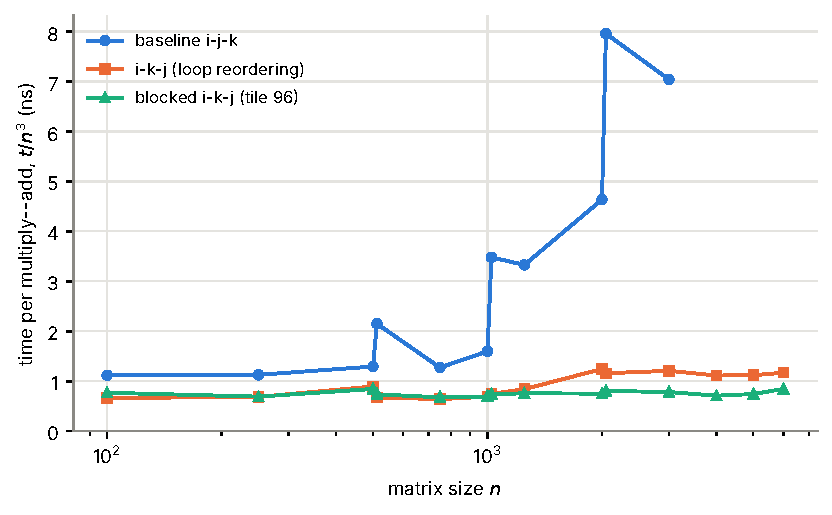
\includegraphics[width=.8\textwidth]{../figures/fig2_dense_normalised.pdf}
\caption{Time per multiply--add, $t/n^3$, against $n$ (median; the IQR is smaller than the markers except at a few sizes, see Table~\ref{tab:dense}).}
\label{fig:norm}
\end{figure}

\paragraph{Loop reordering and blocking.} The baseline costs $1.1$--$1.6$\,ns per multiply--add for $n\le1000$ except at $n=512$ ($2.15$\,ns), and then rises to
$3.5$\,ns at $1024$, $3.3$ at $1250$, $4.6$ at $2000$, $8.0$ at $2048$ and $7.0$ at $3000$ (Figure~\ref{fig:norm}), as in Assignment~1. i-k-j costs $0.64$--$0.89$\,ns up to $n=1250$ and
$1.1$--$1.24$\,ns from $n=2000$; it shows \emph{no} spike at $512$ or $1024$. The blocked method stays between $0.68$ and $0.85$\,ns at \emph{all} sizes up to $6000$.
The speed-up of i-k-j over the baseline is $1.45$--$1.69\times$ for $n\le500$, $2.0$--$2.3\times$ at $750$ and $1000$, and $3.7$--$6.9\times$ for $n\ge1024$ (Figure~\ref{fig:speed});
for the blocked method it is $9.9\times$ at $2048$ and $9.0\times$ at $3000$. The speed-ups are not monotonic in $n$ because the \emph{baseline} is the irregular series:
the largest values ($3.2\times$ at $512$, $4.7\times$ at $1024$, $6.9\times$ and $9.9\times$ at $2048$) coincide with sizes where the baseline itself is anomalously slow, so they partly measure that anomaly.
The blocked method is not faster than i-k-j for $n\le1000$ ($1.00\times$ at $1000$) and gains $1.11\times$ at $1250$, $1.66\times$ at $2000$, $1.44\times$ at $2048$, $1.54\times$ at $3000$, $1.57\times$ at $4000$, $1.51\times$ at $5000$ and $1.38\times$ at $6000$.

\begin{figure}[H]
\centering
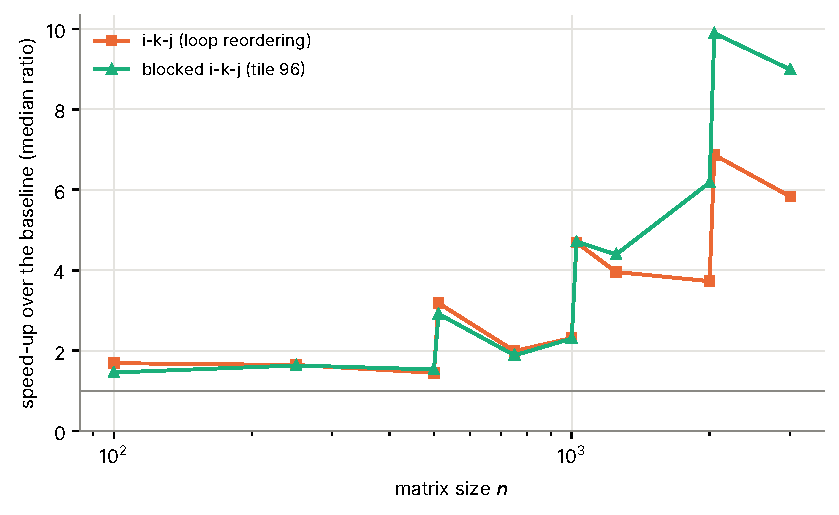
\includegraphics[width=.8\textwidth]{../figures/fig3_dense_speedup.pdf}
\caption{Speed-up over the i-j-k baseline (median ratio). The baseline is measured with only $2$--$5$ samples for $n\ge750$.}
\label{fig:speed}
\end{figure}

\paragraph{Empirical exponents.} Fitting $t\propto n^k$ by least squares in log--log (Table~\ref{tab:fit}; $\pm$ is the $95\%$ confidence interval of the slope, few points, so it is rough):
the blocked method has $k=3.04\pm0.07$ over all feasible $n\ge1000$ (nine sizes), i-k-j $3.26\pm0.19$, and the baseline $4.1\pm1.0$ over $1000$--$3000$ (six points that include the spikes).

\begin{table}[H]
\centering\small
\begin{tabular}{lccc}
\toprule
Method & $n=100$--$500$ & $n=1000$--$3000$ & $n\ge1000$ (all feasible) \\
\midrule
baseline i-j-k & $3.09 \pm 0.68$ (3) & $4.11 \pm 0.97$ (6) & $4.11 \pm 0.97$ (6) \\
i-k-j (loop reordering) & $3.18 \pm 1.23$ (3) & $3.56 \pm 0.28$ (6) & $3.26 \pm 0.19$ (9) \\
blocked i-k-j (tile 96) & $3.05 \pm 1.45$ (3) & $3.09 \pm 0.10$ (6) & $3.04 \pm 0.07$ (9) \\
\bottomrule
\end{tabular}

\caption{Fitted exponent $k$ of $t\propto n^k$ with the $95\%$ CI of the slope and the number of points.}
\label{tab:fit}
\end{table}

\paragraph{Largest feasible size, budget and memory.}
\begin{table}[H]
\centering\scriptsize
\resizebox{\textwidth}{!}{\begin{tabular}{lrrlrrl}
\toprule
Method & Largest feasible $n$ & Largest attempted $n$ & Failures (limit 300 s) & Time at largest ok (s) & Reps & Not attempted \\
\midrule
baseline i-j-k & 3000 & 4000 & 4000: timeout & 190 & 2 & 5000, 6000, 8000 \\
i-k-j (loop reordering) & 6000 & 8000 & 8000: timeout & 253 & 2 & none \\
blocked i-k-j (tile 96) & 6000 & 8000 & 8000: timeout & 183 & 2 & none \\
\bottomrule
\end{tabular}
}
\caption{Largest feasible and largest attempted size under the budgets (300\,s per sample, 4\,GiB). \emph{Not attempted}: skipped after an earlier timeout of the same series.}
\label{tab:limits}
\end{table}
The baseline completes $n=3000$ ($190$\,s) and times out at $4000$; i-k-j and blocked complete $6000$ ($253$\,s and $183$\,s, two samples each) and time out at $8000$.
All limits are set by \emph{time}, not by memory: the largest dense run used $826$\,MiB (Table~\ref{tab:mem}). Peak RSS grows by $24.00$ bytes per $n^2$ in all three methods (three \texttt{float64} matrices, H6)
above a baseline of about $2$\,MiB, and equals the $24n^2$ model within $0.3\%$ at the largest size.

\begin{table}[H]
\centering\scriptsize
\resizebox{\textwidth}{!}{\begin{tabular}{lrrrrr}
\toprule
Method & Peak RSS at $n=100$ (MiB) & Growth (bytes per $n^2$, $n\ge1000$) & Largest $n$ & Peak RSS there (MiB) & $24n^2$ model (MiB) \\
\midrule
baseline i-j-k & 2.00 & 24.00 & 3000 & 207.8 & 206.0 \\
i-k-j (loop reordering) & 2.00 & 24.00 & 6000 & 825.8 & 824.0 \\
blocked i-k-j (tile 96) & 2.00 & 24.00 & 6000 & 825.8 & 824.0 \\
\bottomrule
\end{tabular}
}
\caption{Peak resident memory of the dense methods (\texttt{VmHWM}) and the model $24n^2$ bytes.}
\label{tab:mem}
\end{table}

\paragraph{Bottleneck.} At $n\ge2000$ the baseline spends $4.6$--$8.0$\,ns per multiply--add, $4$--$12$ times the $0.64$--$0.89$\,ns of the unit-stride methods, i.e.\ most of its time is memory access and not arithmetic.
For the unit-stride methods the cost rises from about $0.7$ to $1.1$--$1.2$\,ns for i-k-j when the matrices no longer fit in the caches ($n\ge2000$: $B$ alone is $32$\,MB, much larger than the $1$\,MiB L2), while blocking holds $0.7$--$0.85$\,ns. This is consistent with a cache-capacity effect but, since no hardware counters
are available in the virtual machine, it is an \emph{interpretation}, not a measurement.

\subsection{Tile size, compiler options and variability (supplementary, kept separate)}
\label{sec:resbs}
\begin{table}[H]
\centering\small
\begin{tabular}{rrrrr}
\toprule
Tile $b$ & Process 1 (s) & Process 2 (s) & Mean (s) & $3\cdot8b^2$ (KiB) \\
\midrule
8 & 2.76 & 2.98 & 2.87 & 1.50 \\
16 & 2.54 & 2.77 & 2.65 & 6.00 \\
24 & 2.50 & 2.97 & 2.73 & 13.5 \\
32 & 2.54 & 2.72 & 2.63 & 24.0 \\
48 & 2.76 & 2.75 & 2.76 & 54.0 \\
64 & 2.50 & 2.63 & 2.56 & 96.0 \\
\textbf{96} & 2.47 & 2.53 & \textbf{2.50} & 216 \\
128 & 2.79 & 2.40 & 2.60 & 384 \\
192 & 2.83 & 2.49 & 2.66 & 864 \\
256 & 2.93 & 2.49 & 2.71 & 1536 \\
384 & 2.92 & 2.74 & 2.83 & 3456 \\
\bottomrule
\end{tabular}

\caption{Tile-size sweep of the blocked method at $n=1500$ (seconds, median of two independent processes and their mean). Best tile in bold.}
\label{tab:bs}
\end{table}
The mean time is lowest at $b=96$ ($2.50$\,s), but the whole range $b=16$--$256$ lies within $2.50$--$2.76$\,s ($\le10\%$) and the two processes disagree by up to $0.5$\,s at the same tile size ($b=24$: $2.50$ versus $2.97$\,s); $b=8$ and $b=384$ are $13$--$15\%$ slower.
The landscape is therefore flat and $b=96$ is a reasonable but not a uniquely optimal choice (Figure~\ref{fig:tile}).

\begin{figure}[H]
\centering
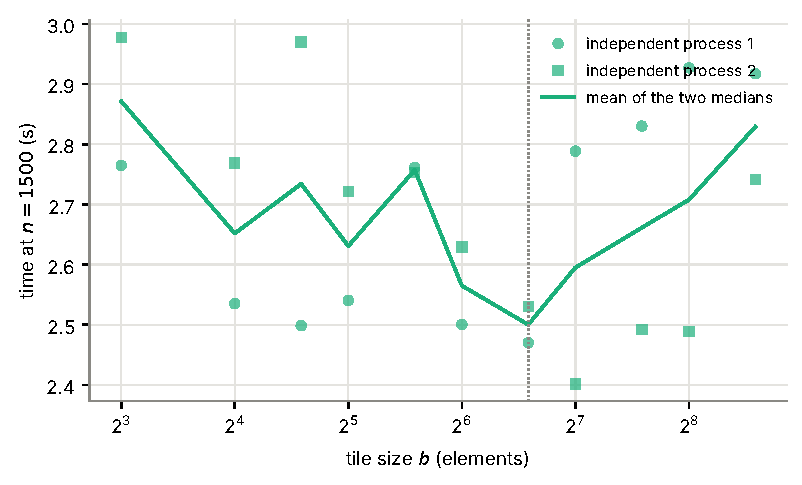
\includegraphics[width=.62\textwidth]{../figures/fig5_tile_sweep.pdf}
\caption{Blocked method at $n=1500$ against the tile size, two processes.}
\label{fig:tile}
\end{figure}

\paragraph{Between-process variability.}\label{sec:resproc} Repeating the same configuration at $n=1000$ in six independent processes (Table~\ref{tab:procvar}) gives medians that differ by $14\%$ (i-k-j), $13\%$ (blocked) and $35\%$ (baseline) from the fastest to the slowest process, which is of the same size as, or larger than,
the within-process IQR ($9$--$14\%$ of the median). Differences between methods or settings below roughly $15\%$ must not be read as real; for the baseline, $35\%$.

\begin{table}[H]
\centering\scriptsize
\begin{tabular}{lrrrrrrrrr}
\toprule
Method & Proc. & P1 (s) & P2 (s) & P3 (s) & P4 (s) & P5 (s) & P6 (s) & Spread (\%) & Within IQR (\%) \\
\midrule
baseline i-j-k & 6 & 1.60 & 1.65 & 2.12 & 1.75 & 1.65 & 1.54 & 35.1 & 9.23 \\
i-k-j (loop reordering) & 6 & 0.690 & 0.724 & 0.753 & 0.795 & 0.738 & 0.728 & 14.3 & 11.1 \\
blocked i-k-j (tile 96) & 6 & 0.695 & 0.758 & 0.775 & 0.789 & 0.734 & 0.752 & 12.5 & 14.0 \\
\bottomrule
\end{tabular}

\caption{Median time at $n=1000$ in six independent processes; spread = (max $-$ min)/min.}
\label{tab:procvar}
\end{table}

\paragraph{Compiler options (Section~\ref{sec:supp}).}
\label{sec:resflags}
\begin{table}[H]
\centering\scriptsize
\begin{tabular}{rlrrrr}
\toprule
$n$ & method & \texttt{-O2} (s) & \texttt{-O2 -funroll-loops} & \texttt{-O3} & \texttt{-O3 -march=native} \\
\midrule
1000 & blocked & 0.865 & 0.495 (1.75$\times$) & 0.242 (3.57$\times$) & 0.232 (3.73$\times$) \\
1000 & ijk & 1.89 & 1.60 (1.18$\times$) & 1.69 (1.11$\times$) & 1.58 (1.19$\times$) \\
1000 & ikj & 0.833 & 0.492 (1.69$\times$) & 0.341 (2.44$\times$) & 0.283 (2.94$\times$) \\
2000 & blocked & 5.99 & 4.02 (1.49$\times$) & 2.59 (2.31$\times$) & 1.83 (3.27$\times$) \\
2000 & ijk & 36.6 & 33.8 (1.08$\times$) & 37.3 (0.98$\times$) & 36.1 (1.02$\times$) \\
2000 & ikj & 9.08 & 8.67 (1.05$\times$) & 6.20 (1.46$\times$) & 5.84 (1.55$\times$) \\
\bottomrule
\end{tabular}

\caption{Median time (s) of each method with other compiler options (in parentheses, speed-up over the same method at \texttt{-O2} in the same experiment; always \texttt{-ffp-contract=off}).}
\label{tab:flags}
\end{table}
At \texttt{-O2} gcc does not vectorise any kernel (no packed multiplication in the object code, \texttt{results/vectorization\_evidence.csv}); at \texttt{-O3} it emits packed multiplications for i-k-j and blocked (128-bit registers; 256-bit with \texttt{-march=native}) and a single one for the baseline, whose inner loop reads a column of $B$ with a stride, and its time does not change. The effect is large:
at $n=1000$ the blocked kernel at \texttt{-O3} is $3.6\times$ faster than at \texttt{-O2}, and at $n=2000$ \texttt{-O3 -march=native} makes blocked $3.3\times$ and i-k-j $1.55\times$ faster, while the baseline does not change ($0.98$--$1.02\times$; the $1.08\times$ of unrolling
is below the variability). The \texttt{-O2} values of this table ($0.83$/$0.87$/$1.89$\,s at $n=1000$) are from a different process than those of Table~\ref{tab:dense} ($0.69$/$0.70$/$1.60$\,s), an instance of the variability above.
The headline comparison of this report uses \texttt{-O2} for all methods; a compiler flag is therefore a larger optimisation than blocking at $n=1000$, and at $n=2000$ it is of the same order.

\subsection{Part B: sparse matrices}

\paragraph{Inputs.} Table~\ref{tab:sparse2000} (and the same tables for $n=500$ and $1000$ in the materials) lists, for each density, the achieved density of the inputs, the density of the product $C$, the CSR kernel time, the separately timed
dense$\to$CSR conversion (both $A$ and $B$), the time of the best dense method of the same cell and of the baseline, and the speed-ups of the CSR kernel $S_k$ and of kernel plus conversion $S_t$ over the best dense method.
Dense times of the same method vary between cells only within the variability above ($0.69$--$0.82$\,s for i-k-j at $n=1000$, $8.4$--$10.1$\,s at $n=2000$, with no trend in density): \emph{the dense methods do not depend on the values}, which also confirms that the comparison base is the same for all densities.

\begin{table}[H]
\centering\scriptsize
\begin{tabular}{lrrrrrrrrr}
\toprule
Input & $d$ (\%) & actual (\%) & $C$ (\%) & CSR kernel (s) & conv. (s) & best dense (s) & i-j-k (s) & $S_k$ & $S_t$ \\
\midrule
random & 0.100 & 0.0998 & 0.199 & 0.000135 & 0.0236 & 5.97 & -- & 44235 & 251 \\
 & 1.00 & 1.00 & 18.2 & 0.0203 & 0.0230 & 6.52 & -- & 322 & 151 \\
 & 5.00 & 5.00 & 99.3 & 0.137 & 0.0303 & 6.59 & -- & 48.2 & 39.4 \\
 & 10.0 & 10.0 & 100 & 0.164 & 0.0315 & 6.26 & -- & 38.3 & 32.1 \\
 & 20.0 & 20.0 & 100 & 0.446 & 0.0448 & 6.11 & -- & 13.7 & 12.4 \\
 & 30.0 & 30.0 & 100 & 1.02 & 0.0558 & 6.04 & -- & 5.95 & 5.64 \\
 & 50.0 & 50.0 & 100 & 3.15 & 0.0741 & 5.84 & 35.8 & 1.86 & 1.81 \\
 & 70.0 & 70.0 & 100 & 5.64 & 0.0715 & 6.01 & -- & 1.07 & 1.05 \\
 & 90.0 & 90.0 & 100 & 9.44 & 0.0645 & 5.81 & -- & 0.615 & 0.611 \\
\midrule
band & 0.100 & 0.1000 & 0.150 & 0.0000410 & 0.0205 & 5.90 & 35.5 & 143712 & 287 \\
 & 1.00 & 0.998 & 1.94 & 0.00191 & 0.0223 & 6.41 & -- & 3358 & 265 \\
 & 5.00 & 4.99 & 9.80 & 0.0222 & 0.0242 & 5.90 & -- & 265 & 127 \\
 & 10.0 & 9.99 & 19.4 & 0.0839 & 0.0252 & 6.10 & -- & 72.7 & 55.9 \\
 & 20.0 & 20.0 & 37.7 & 0.318 & 0.0274 & 5.84 & -- & 18.4 & 16.9 \\
 & 30.0 & 30.0 & 54.6 & 0.720 & 0.0322 & 6.09 & -- & 8.45 & 8.09 \\
 & 50.0 & 50.0 & 82.8 & 2.03 & 0.0410 & 5.74 & -- & 2.83 & 2.77 \\
 & 70.0 & 70.0 & 99.1 & 4.94 & 0.0437 & 6.18 & -- & 1.25 & 1.24 \\
 & 90.0 & 90.0 & 100 & 9.05 & 0.0486 & 5.81 & -- & 0.643 & 0.639 \\
\bottomrule
\end{tabular}

\caption{$n=2000$: CSR$\times$CSR versus the best dense method (blocked). $d$ = density of the inputs (\% nonzero); ``actual'' = measured; $C$ = density of the product. Times in seconds; ``--'' = not run (baseline only at two cells).
$S_k=t_{dense}/t_{kernel}$, $S_t=t_{dense}/(t_{kernel}+t_{conv})$.}
\label{tab:sparse2000}
\end{table}

\begin{figure}[H]
\centering
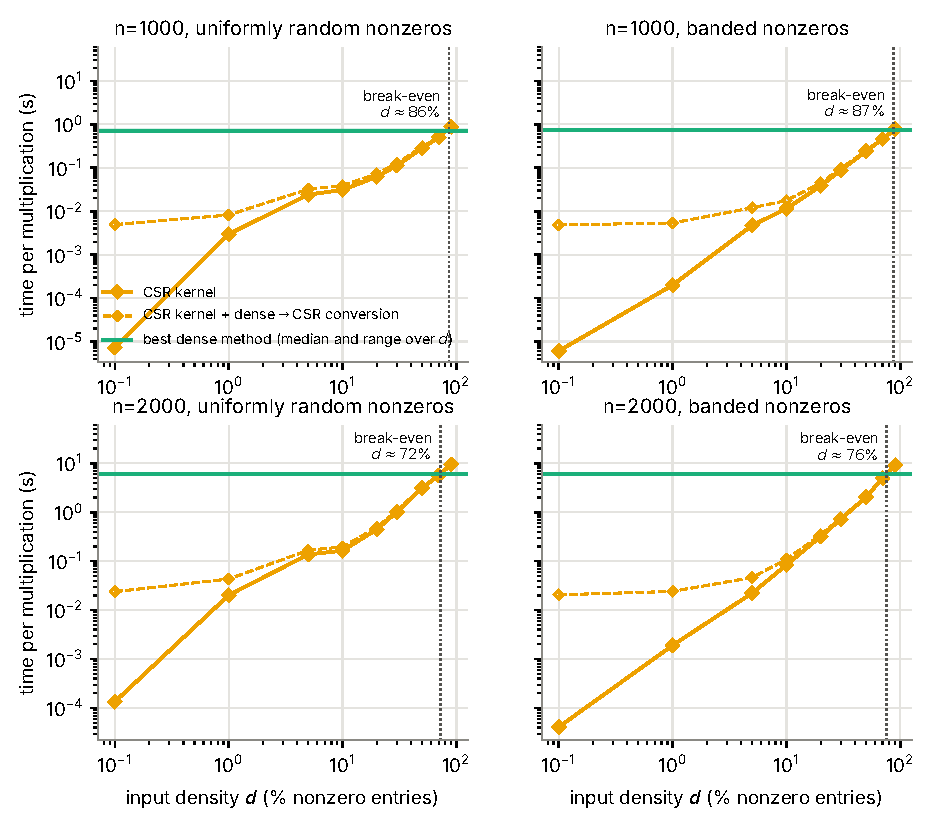
\includegraphics[width=\textwidth]{../figures/fig7_sparse_vs_dense.pdf}
\caption{Time per multiplication of the CSR kernel (with and without the dense$\to$CSR conversion) against the input density $d$. The dense methods do not depend on $d$, so only the best one is drawn: its median over the densities (line) and its range (shaded). The dotted line marks the interpolated break-even density of the kernel. All three dense methods are listed in Table~\ref{tab:sparse2000}.}
\label{fig:sparse}
\end{figure}

\paragraph{Where sparse wins.} At $d=0.1\%$ and $n=1000$ the CSR kernel takes $7.3\,\mu$s (random) and $6.1\,\mu$s (banded), against $0.69$--$0.75$\,s of the best dense method, a ratio of $10^5$; at $n=2000$ the ratios are $4\cdot10^4$ (random) and $1.4\cdot10^5$ (banded).
The advantage falls steadily with density (Figure~\ref{fig:sparse}), is still $1.9$--$3.1\times$ at $d=50\%$ and disappears near the top of the range: the speed-up of the kernel at the largest density tested ($90\%$) is $0.82$--$0.93$ for $n\le1000$ and $0.62$--$0.64$ for $n=2000$; the break-even density, by log--log interpolation
between the neighbouring tested densities, is $82$--$87\%$ for $n=500,1000$ and $72$--$76\%$ for $n=2000$ (\texttt{results/summary\_breakeven.csv}, kernel only; with conversion, $0.2$--$2$ points lower). Because the ratios near $1$ are within the variability ($\pm15\%$), the break-even at $n\le1000$ is only
resolved to about $\pm10$ percentage points; the result at $n=2000$ ($0.61$--$0.64$ at $90\%$) is outside that margin.

\paragraph{Conversion.} Converting two dense matrices to CSR costs $4.8$--$21$\,ms at $n=1000$ and $21$--$74$\,ms at $n=2000$ (it grows with the number of nonzeros, from the minimum at $d=0.1\%$). For $d\le1\%$ banded it is $92$--$99.9\%$ of the end-to-end sparse time (e.g.\ $n=1000$, $d=0.1\%$: kernel $6\,\mu$s, conversion $4.8$\,ms), so the end-to-end advantage is $155\times$ rather than $10^5\times$ (H5 supported);
it falls below $5\%$ of the total for $d\ge70\%$ at $n=1000$ and for $d\ge50\%$ at $n=2000$. If the matrices are already in CSR the conversion does not exist, which is the case of the scaling runs below.

\paragraph{Output density and indexing.} The product of random matrices fills in: at $n=1000$, $C$ has $0.10\%$ of nonzeros for $d=0.1\%$, $9.4\%$ for $d=1\%$, $91.7\%$ for $d=5\%$ and $100\%$ from $d=10\%$, in line with $1-e^{-nd^2}$ ($9.5\%$, $91.8\%$ and $100\%$ predicted) (Figure~\ref{fig:fill}). The product of banded matrices stays banded,
with density $\approx2d$ ($1.9\%$ at $d=1\%$, $19\%$ at $d=10\%$). The cost per useful product of the CSR kernel, $t/\text{flops}$ with flops $=\sum_k\mathrm{colcount}_A(k)\,\mathrm{rowcount}_B(k)$ (Table~\ref{tab:nsflop}), is $0.9$--$1.1$\,ns for banded inputs with $d\ge10\%$ at $n=1000$ (the same order as the dense $0.7$--$0.8$\,ns per
multiply--add) but $30$\,ns for random inputs at $d=1\%$ ($n=1000$) and $25$\,ns at $n=2000$, falling to $9.7$\,ns at $5\%$, $3.1$\,ns at $10\%$ and $1.1$\,ns at $50\%$. In the same density ($1\%$) random and banded inputs differ by $15\times$ in kernel time (3.0\,ms versus 0.20\,ms at $n=1000$) and by $15\times$ in cost per flop.
Hence \emph{the density alone does not determine the performance}: the structure changes the number of useful products, the access pattern to the output workspace, the size of the output and the cost of the column sort. The mechanisms by which random access to a length-$n$ workspace and output growth increase the cost per flop are plausible hypotheses (cache and TLB misses, sorting, \texttt{realloc}), not measured here.

\begin{figure}[H]
\centering
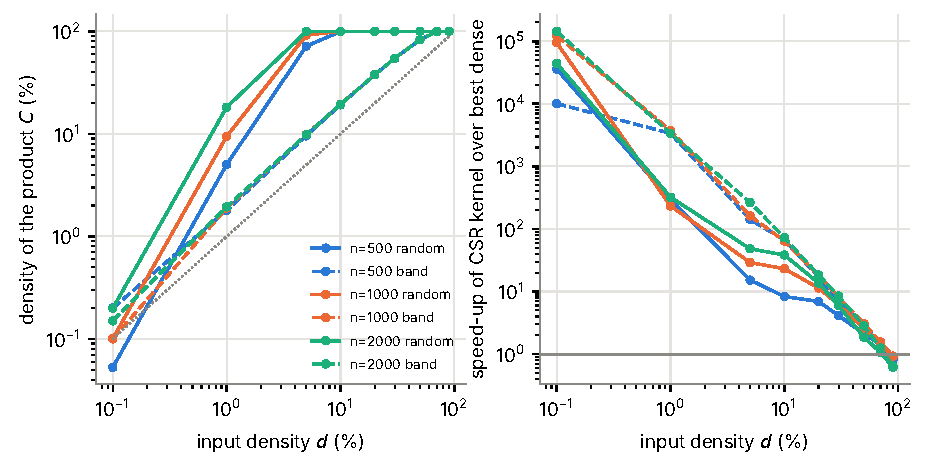
\includegraphics[width=\textwidth]{../figures/fig8_sparse_speedup_output_density.pdf}
\caption{Left: density of the product against input density; the dotted line is $y=x$. Right: speed-up of the CSR kernel over the best dense method (horizontal line: 1).}
\label{fig:fill}
\end{figure}

\begin{table}[H]
\centering\scriptsize
\begin{tabular}{rllrrrr}
\toprule
$n$ & input & $d$ (\%) & $1$ & $5$ & $10$ & $50$ \\
\midrule
1000 & random & ns/flop & 30.0 & 9.66 & 3.13 & 1.12 \\
1000 & banded & ns/flop & 2.00 & 1.87 & 1.13 & 0.93 \\
2000 & random & ns/flop & 25.2 & 6.84 & 2.05 & 1.58 \\
2000 & banded & ns/flop & 2.40 & 1.11 & 1.04 & 0.98 \\
\bottomrule
\end{tabular}
\caption{Cost per useful product of the CSR kernel (ns per flop, flops counted from the CSR operands) at selected densities; the conversion is not included.}
\label{tab:nsflop}
\end{table}

\paragraph{Memory.} The sparse method \emph{csr} holds the dense inputs (to convert them each repetition) and the CSR copies and the output; its peak RSS at $n=2000$ is $63$--$78$\,MiB for $d\le1\%$ but $164$--$200$\,MiB when the product is dense, versus $93$\,MiB for the dense methods (Table~\ref{tab:sparsemem}).
The CSR storage model $12$ bytes per nonzero of $A$, $B$ and $C$ plus $24(n+1)$ matches the measured resident memory of the CSR-only runs (below) within $1\%$ at the sizes with $n\ge32000$ ($d=0.1\%$) and $n\ge8000$ ($d=1\%$).

\begin{table}[H]
\centering\scriptsize
\begin{tabular}{lrrrrr}
\toprule
Input & $d$ (\%) & $C$ (\%) & CSR storage of $A,B,C$ (MiB) & peak RSS sparse (MiB) & peak RSS dense (MiB) \\
\midrule
random & 0.100 & 0.199 & 0.229 & 63.1 & 93.3 \\
 & 1.00 & 18.2 & 9.29 & 78.2 & 93.3 \\
 & 5.00 & 99.3 & 50.1 & 166 & 93.3 \\
 & 10.0 & 100 & 55.0 & 182 & 93.3 \\
 & 20.0 & 100 & 64.1 & 182 & 93.3 \\
 & 30.0 & 100 & 73.3 & 164 & 93.3 \\
 & 50.0 & 100 & 91.6 & 200 & 93.3 \\
 & 70.0 & 100 & 110 & 173 & 93.3 \\
 & 90.0 & 100 & 128 & 191 & 93.3 \\
\midrule
band & 0.100 & 0.150 & 0.206 & 63.0 & 93.3 \\
 & 1.00 & 1.94 & 1.85 & 64.7 & 93.3 \\
 & 5.00 & 9.80 & 9.10 & 71.9 & 93.3 \\
 & 10.0 & 19.4 & 18.1 & 80.9 & 93.3 \\
 & 20.0 & 37.7 & 35.6 & 98.4 & 93.3 \\
 & 30.0 & 54.6 & 52.5 & 115 & 93.3 \\
 & 50.0 & 82.8 & 83.8 & 147 & 93.3 \\
 & 70.0 & 99.1 & 109 & 172 & 93.3 \\
 & 90.0 & 100 & 128 & 191 & 93.3 \\
\bottomrule
\end{tabular}

\caption{$n=2000$: CSR storage of $A$, $B$, $C$ (model) and peak RSS of the \emph{csr} method (dense inputs resident) and of the dense methods.}
\label{tab:sparsemem}
\end{table}

\paragraph{Scaling with CSR inputs and the budget.} With inputs already in CSR (random, \emph{csrfile}) the sizes of Table~\ref{tab:scale} were run. At $d=0.1\%$ the sequence reached $n=64000$ ($14$\,s, $2.9$\,GiB, product density $6.2\%$, $254$ million nonzeros); at $d=1\%$ it reached $n=16000$ ($4.3$\,s, $2.3$\,GiB, product density $80\%$).
The next sizes ($n=128000$ at $0.1\%$, $n=32000$ at $1\%$) were \emph{not attempted} because the predicted memory ($47.6$ and $23.8$\,GB) is more than three times the budget: \textbf{no sparse run hit a real failure}; the limit reported is the largest feasible size, and the next size is excluded by prediction, not by an observed failure.
The time grows as $n^{3.4}$ at $d=0.1\%$ and $n^{2.6}$ at $d=1\%$ over the measured sizes, while the number of useful products grows as $n^{3.0}$ at fixed density, so the cost per flop is not constant ($15$--$69$\,ns at $0.1\%$, $10$--$26$\,ns at $1\%$); memory is dominated by the output, which grows faster than the inputs ($\propto n^{2.5}$ at the largest sizes) because of the fill-in.
For comparison, a dense $n=64000$ product would need $24n^2=98$\,GB (computed, not measured), and the dense methods stopped at $6000$ because of time.

\begin{table}[H]
\centering\scriptsize
\begin{tabular}{rrrrrrrrr}
\toprule
$d$ (\%) & $n$ & nnz($A$) & nnz($C$) & $C$ dens. (\%) & time (s) & reps & peak RSS (MiB) & CSR est. (MiB) \\
\midrule
0.100 & 2000 & 3.99e+03 & 7.97e+03 & 0.199 & 0.000119 & 10 & 2.023 & 0.2286 \\
 & 4000 & 1.63e+04 & 6.52e+04 & 0.407 & 0.00192 & 10 & 4.145 & 1.207 \\
 & 8000 & 6.41e+04 & 5.09e+05 & 0.796 & 0.0295 & 10 & 13.75 & 7.476 \\
 & 16000 & 2.57e+05 & 4.09e+06 & 1.60 & 0.278 & 10 & 96.10 & 52.99 \\
 & 32000 & 1.02e+06 & 3.22e+07 & 3.14 & 2.26 & 5 & 394.6 & 392.5 \\
 & 64000 & 4.1e+06 & 2.54e+08 & 6.20 & 14.0 & 5 & 3004 & 3002 \\
 & 128000 & -- & -- & -- & \emph{not attempted} & -- & -- & -- \\
\midrule
1.00 & 2000 & 4e+04 & 7.28e+05 & 18.2 & 0.0205 & 10 & 17.21 & 9.292 \\
 & 4000 & 1.6e+05 & 5.26e+06 & 32.9 & 0.109 & 10 & 65.84 & 64.00 \\
 & 8000 & 6.39e+05 & 3.52e+07 & 55.1 & 0.811 & 5 & 420.0 & 418.1 \\
 & 16000 & 2.56e+06 & 2.04e+08 & 79.8 & 4.29 & 5 & 2398 & 2396 \\
 & 32000 & -- & -- & -- & \emph{not attempted} & -- & -- & -- \\
\bottomrule
\end{tabular}

\caption{Scaling of the CSR kernel with CSR inputs (random, $d=0.1\%$ and $1\%$). Time = median of the kernel (conversion not applicable); peak RSS measured; CSR est. = $12(\text{nnz}_A+\text{nnz}_B+\text{nnz}_C)+24(n+1)$ bytes.}
\label{tab:scale}
\end{table}

\begin{figure}[H]
\centering
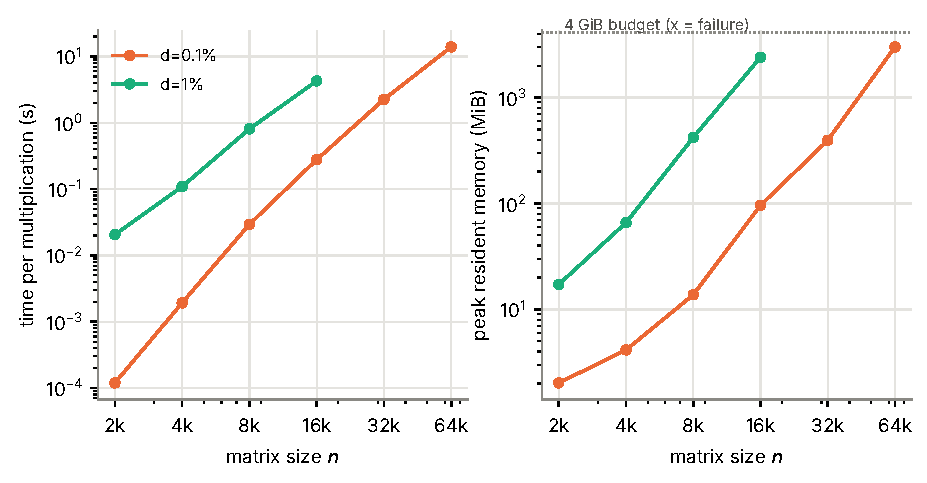
\includegraphics[width=\textwidth]{../figures/fig9_sparse_scaling.pdf}
\caption{Time and peak memory of the CSR kernel against $n$ with CSR inputs. The dotted line is the $4$\,GiB budget; no run failed.}
\label{fig:scale}
\end{figure}

\subsection{Correctness tests}
\begin{table}[H]
\centering\small
\begin{tabular}{lrr}
\toprule
Group of tests & Checks & Passed \\
\midrule
Dense: known answers (scalar, 2$\times$2, 3$\times$3, zero, identity, all-ones, integer) & 117 & 117 \\
Dense: random matrices vs NumPy ($n=5,\dots,129$) & 78 & 78 \\
Dense: bit-for-bit equality of all methods and 13 tile sizes & 13 & 13 \\
Dense: repeated runs give identical checksums & 7 & 7 \\
Sparse: edge cases (empty, identity, diagonal, empty row/column, $1\times1$, fully dense) & 64 & 64 \\
Sparse: random and banded vs SciPy (pattern, values), CSR sorted, csr$=$csrfile & 72 & 72 \\
Sparse: densified result bit-for-bit equal to the dense methods & 24 & 24 \\
Sparse: conversion, spot-check rows, repeated runs & 2 & 2 \\
\midrule
\textbf{Total} & \textbf{377} & \textbf{377} \\
\bottomrule
\end{tabular}

\caption{Results of the correctness suite (run before the benchmarks and again before submission).}
\label{tab:tests}
\end{table}

\section{Discussion}

\subsection{Answers to the research questions}

\paragraph{Q-A (dense optimisations).} With identical inputs, arithmetic, timing boundary and a single thread, reordering the loops to i-k-j makes the C baseline $1.5$--$1.7\times$ faster for $n\le500$, $2$--$2.3\times$ at $n=750$--$1000$ and $3.7$--$6.9\times$
for $n\ge1024$; blocking with $b=96$ adds nothing up to $n=1000$ and a further $1.4$--$1.7\times$ over i-k-j for $n\ge2000$, giving up to $9.9\times$ over the baseline at $n=2048$ (Table~\ref{tab:dense}, Figure~\ref{fig:speed}). The optimised kernels cost
$0.64$--$0.89$\,ns (i-k-j, $n\le1250$) or $0.68$--$0.85$\,ns (blocked, all sizes) per multiply--add and keep a near-cubic growth ($k=3.04\pm0.07$ for blocked), whereas the baseline's cost per multiply--add grows from $1.1$ to $8.0$\,ns. As a consequence the largest feasible size under the same budget moves from $3000$ to $6000$.
The speed-up numbers are bounded by the baseline's irregular behaviour (spikes at $512$ and $1024$): they should be read as ``at these sizes'' and not as a smooth law.

\paragraph{Q-B (sparse versus dense).} For inputs with $0.1$--$50\%$ nonzeros the own CSR$\times$CSR kernel is faster than the best dense method on the same matrices, by $10^5\times$ at $d=0.1\%$ (kernel only), $2\cdot10^2$--$4\cdot10^3\times$ at $1\%$ and $2$--$3\times$ at $50\%$; it is slower from a break-even density of about $72$--$87\%$ (precisely: $72$--$76\%$ at $n=2000$; $82$--$87\%$ at $n=500$ and $1000$, resolved to about $\pm10$ points).
The end-to-end advantage of the whole pipeline starting from dense matrices is limited by the dense$\to$CSR conversion ($O(n^2)$ and independent of $d$ to first order): at $n=1000$, $d=0.1\%$ it is $155\times$ instead of $10^5\times$. And the product of random sparse matrices is dense long before the inputs are: at $n=1000$, $d=5\%$ gives a $92\%$-dense $C$, and then
the cost per useful product ($9.7$\,ns at $5\%$, $30$\,ns at $1\%$) is $14$--$43\times$ that of a dense multiply--add ($0.7$\,ns; Table~\ref{tab:nsflop}). \emph{Where sparse helps}: very sparse inputs, banded or otherwise structured inputs whose product stays sparse, and inputs that are already stored in CSR. \emph{Where it stops helping}: dense outputs, inputs above $\approx70$--$80\%$ density, and
workloads that must convert from dense each time.

\paragraph{Separating the effects.} The optimisation effect (Part~A) was obtained with dense inputs, where the number of operations is fixed at $n^3$: changing the loop order or blocking changed the time by up to $9.9\times$ and nothing else. The storage and structure effect (Part~B) is of a different kind: it changes the \emph{number} of operations (from $n^3$ to $\approx d^2n^3$ useful products for random inputs),
by up to $10^5\times$, while the time per operation \emph{increases} ($1$ to $30$\,ns per product instead of $0.7$\,ns). The two are not additive: here the comparator in Part~B is the best optimised dense method, not the baseline; against the baseline all sparse speed-ups would be about $2\times$ ($n=1000$) to $6\times$ ($n=2000$) larger (baseline column of the tables). Also the
third factor, the \emph{compiler}, matters: with \texttt{-O3 -march=native} the dense blocked kernel became $3.3\times$ faster at $n=2000$, which would move the break-even density of Part~B down (the sparse kernel was not recompiled in the same comparison, so this is only an expectation).

\paragraph{Percentage of zeros is not enough.} At the same $d=1\%$ and $n=1000$, banded inputs run $15\times$ faster than random ones, produce a product $5\times$ sparser ($1.9\%$ versus $9.4\%$), and have $15\times$ lower cost per useful product. A statement such as ``a matrix with $99\%$ zeros is fast'' is therefore false in general: it depends on the pattern,
on the product's fill-in, on the format, on whether conversion is needed and on the implementation of the kernel.

\paragraph{Why a tile of 96 works although it does not fit in L1.} Three $96\times96$ tiles occupy $216$\,KiB, far more than the $32$\,KiB L1 data cache, yet $b=96$ was not slower than $b=32$ (which fits; $2.50$ versus $2.63$\,s, within the variability). The three-tiles-in-L1 criterion of Section~2 is conservative for this loop order: inside a tile the i-k-j order only needs one row of the $C$ tile and one row of the $B$ tile at a time ($768$\,bytes each) in L1, while the $B$ tile ($72$\,KiB) is reused from L2 for every row $i$ and is read with unit stride, a pattern the hardware prefetchers predict well. This explanation is a hypothesis; without hardware counters it was not measured.

\subsection{Hypotheses}
\begin{table}[H]
\centering\small
\begin{tabular}{@{}p{0.6cm}p{3.1cm}p{10.2cm}@{}}
\toprule
 & Verdict & Evidence \\
\midrule
H1 & supported & i-k-j is $1.45$--$6.9\times$ faster than i-j-k at every size; gain grows with $n$ but not monotonically; no spikes at $512$/$1024$. \\
H2 & partly supported & No gain of blocking for $n\le1000$ (as expected); a gain of $1.38$--$1.66\times$ for $n\ge2000$. The predicted bound ``$\lesssim1.5\times$'' is exceeded at $n=2000$ ($1.66\times$) and respected elsewhere. \\
H3 & supported & identical SHA-256 of $C$ in all $69$ groups; all tile sizes tested bit-for-bit equal. \\
H4 & supported, with a precise break-even & $10^5\times$ at $d=0.1\%$ down to $0.6$--$0.9\times$ at $90\%$; break-even $72$--$87\%$; random products fill in as $1-e^{-nd^2}$, banded ones stay banded. \\
H5 & supported & conversion is $92$--$99.9\%$ of the end-to-end time for banded inputs with $d\le1\%$; random $d=1\%$: $53$--$82\%$. \\
H6 & supported & dense: $24.00$ bytes per $n^2$; CSR: model within $1\%$ of the measured RSS at the largest scaling sizes. \\
\bottomrule
\end{tabular}
\caption{Predictions declared in the introduction against the results.}
\end{table}

\subsection{Strength of the evidence}
\begin{itemize}
  \item \textbf{Strong:} the ordering baseline $\ll$ i-k-j $\lesssim$ blocked for $n\ge2000$ (ratios $>3\times$ against samples whose IQR is at most $14\%$ of the median); the correctness of all results; the memory formulas; the orders of magnitude of the sparse advantage at low density, and the fact that it is reversed at $90\%$ for $n=2000$.
  \item \textbf{Moderate:} the break-even densities for $n\le1000$ (the speed-up is within $\pm15\%$ of $1$ over the last two densities); exponents (few points); the choice $b=96$ (flat landscape).
  \item \textbf{Weak or hypothesis:} all explanations in terms of caches, TLB, SIMD units or \texttt{realloc}; they are consistent with the data (e.g.\ the vectorisation evidence and the compiler experiment for SIMD) but no hardware counters were available. For the baseline's spikes at powers of two a cache-associativity conflict is the usual explanation \cite{drepper,hennessy}; this study neither tests nor excludes it.
\end{itemize}

\subsection{Limitations}
\begin{itemize}
  \item \textbf{One machine.} A virtual machine with $2$ vCPUs, $8$\,GiB, shared host, unpinned, no visible frequency governor. Between-process variability reaches $13$--$35\%$ at $n=1000$; with $2$--$5$ samples at large $n$ the medians are less certain than the IQR suggests. Results are \emph{not} from the author's laptop and would differ in absolute terms there.
  \item \textbf{No CPU pinning.} Pinning each process to one logical CPU (\texttt{taskset}) could reduce the between-process noise and will be used in Assignment~3 (threads); in a virtual machine it fixes the process to a vCPU, not to a physical core, so it can reduce but not remove the variability.
  \item \textbf{Few samples at the largest sizes} (budget rule): baseline $n=3000$ has $2$ samples; $4000$--$6000$ have $2$--$3$; the sparse scaling has $5$.
  \item \textbf{Implementation scope.} One sparse format (CSR) and one algorithm (Gustavson with a dense accumulator); no comparison with a library (SciPy was used only to validate), no CSC/COO, no tuned sort. A faster sparse kernel would move the break-even; a library dense kernel (BLAS) would very likely be faster than all three dense methods and would move it down.
  \item \textbf{Inputs.} Two structures only (random and banded) and positive values; real matrices (power-law degree, block structure) may behave differently. Matched comparisons only up to $n=2000$; the baseline is run on only two cells at $n=2000$.
  \item \textbf{Exploratory decisions.} A pilot at $n=1500$ and a smoke test at $n=500$ were seen before the hypotheses were fixed; the densities $70\%$ and $90\%$, the compiler experiment and the variability experiment were added after those looks. The tile was chosen on the same machine at a size outside the comparison.
  \item \textbf{Scaling runs} use CSR files, so they exclude conversion by design, and only random patterns.
\end{itemize}

\section{Conclusions}
\begin{enumerate}
  \item On dense $n\times n$ \texttt{float64} matrices in sequential C at \texttt{-O2}, the i-j-k baseline loses to i-k-j by $1.5\times$ to $6.9\times$, and to the blocked method ($b=96$) by up to $9.9\times$; blocking only pays beyond $n\approx1250$, where it adds $1.4$--$1.7\times$ over i-k-j. The largest feasible size within $300$\,s doubles, from $3000$ to $6000$. Results are bit-identical.
  \item Cost per multiply--add: $0.64$--$0.89$\,ns (i-k-j) and $0.68$--$0.85$\,ns (blocked) against $1.1$--$8.0$\,ns (baseline); exponent $3.04\pm0.07$ (blocked).
  \item The own CSR$\times$CSR kernel is $10^2$--$10^5\times$ faster than the best dense method for $d\le1\%$, still $2$--$3\times$ at $50\%$, and slower above a break-even density of about $70$--$85\%$ on this machine; a dense$\to$CSR conversion removes most of the advantage at high sparsity, and random products become dense after a few percent of input density.
  \item The percentage of zeros alone does not predict performance: at $1\%$, banded inputs are $15\times$ faster than random ones.
  \item With CSR inputs, $n=64000$ ($d=0.1\%$) and $n=16000$ ($d=1\%$) are feasible in $14$\,s and $4.3$\,s within $3$\,GiB; the next sizes were excluded by predicted memory ($>12$\,GiB), and no run failed. Dense matrices of $n=64000$ would need $98$\,GB.
  \item A compiler flag (vectorisation) had an effect comparable to or larger than the algorithmic changes in the dense part ($3.3\times$ for the blocked kernel at $n=2000$); this should be kept in mind when the next assignment adds vectorisation and parallelism.
\end{enumerate}

\section{Use of generative AI}
In line with the course policy, the use of AI is disclosed: the tool was \textbf{Claude (Anthropic)}. It was used for planning the experimental design, writing the C implementations, the input generator, the benchmark driver, the test, analysis and plotting scripts, the supplementary experiments and a first draft of this report.
The affected parts are \texttt{src/}, \texttt{scripts/} and \texttt{report/}. The author is responsible for understanding the code, validating the measurements, checking the references and defending the conclusions; generated text is not evidence, and every number in this report was produced by the included code
from the raw data in \texttt{results/}.

\section{Reproducibility materials}
\label{sec:materials}
Source code, build and run instructions, raw measurements, input-generation scripts and analysis scripts are in the repository \repourl{} and in \path{Assignment02_GonzalezFernandez_Materials.zip}. The \texttt{README.md} gives the exact commands
(\texttt{make build inputs test bench analyze report}); the input matrices are not stored (about $5$\,GB) but regenerated with \texttt{scripts/gen\_inputs.py} and verified against the SHA-256 digests in \texttt{data/manifest.json}; the dense inputs are identical to those of Assignment~1 (\texttt{data/a1\_reference\_sha256.json}).
Raw data: \path{results/raw_measurements.csv} (one row per sample, warm-up included) and \path{results/runs.csv} (one row per process); environment: \path{results/environment.json}; every figure and table is generated by \path{scripts/analyze.py}. The measurement driver reads \texttt{/proc} and therefore needs Linux;
the full campaign took several hours on the reported machine. The baseline kernel is that of Assignment~1 \cite{a1}, whose structure was taken from the example implementations on the course website \cite{course}; all other code, the driver, validation, supplementary experiments and analysis were written for this study with the AI assistance disclosed above.
No other external code, text or figures are reused.

\begin{thebibliography}{99}
\bibitem{a1} H.~Gonz\'alez Fern\'andez, ``Assignment 1: How runtime and memory scale in the basic triple-loop matrix multiplication in C, Java and Python,'' Big Data, Univ. Las Palmas de Gran Canaria, Oct. 2026. Code: \url{https://github.com/hugogzfz/bd-assignment1-matmul}, commit 101af1c.
\bibitem{course} ``Ejemplos'' (matrix-multiplication examples in Python, Java, Rust and C), \emph{Big Data} course website, Block~1, Complexity Management. \url{https://mltechdrawer.github.io/BIGDATA/Block1_Theoretical_Concepts_of_Big_Data/Complexity_Management/codigos/}. Accessed: Oct.~14, 2026.
\bibitem{lam} M.~D.~Lam, E.~E.~Rothberg and M.~E.~Wolf, ``The cache performance and optimizations of blocked algorithms,'' in \emph{Proc. 4th Int. Conf. Architectural Support for Programming Languages and Operating Systems (ASPLOS IV)}, Santa Clara, CA, USA, 1991, pp.~63--74.
\bibitem{goto} K.~Goto and R.~A.~van de Geijn, ``Anatomy of high-performance matrix multiplication,'' \emph{ACM Trans. Math. Softw.}, vol.~34, no.~3, pp.~1--25, 2008.
\bibitem{gustavson} F.~G.~Gustavson, ``Two fast algorithms for sparse matrices: Multiplication and permuted transposition,'' \emph{ACM Trans. Math. Softw.}, vol.~4, no.~3, pp.~250--269, Sep. 1978.
\bibitem{saad} Y.~Saad, \emph{Iterative Methods for Sparse Linear Systems}, 2nd~ed. Philadelphia, PA, USA: SIAM, 2003.
\bibitem{drepper} U.~Drepper, ``What every programmer should know about memory,'' Red~Hat, Inc., Nov. 2007.
\bibitem{hennessy} J.~L.~Hennessy and D.~A.~Patterson, \emph{Computer Architecture: A Quantitative Approach}, 6th~ed. Cambridge, MA, USA: Morgan Kaufmann, 2017.
\bibitem{higham} N.~J.~Higham, \emph{Accuracy and Stability of Numerical Algorithms}, 2nd~ed. Philadelphia, PA, USA: SIAM, 2002.
\bibitem{goldberg} D.~Goldberg, ``What every computer scientist should know about floating-point arithmetic,'' \emph{ACM Comput. Surv.}, vol.~23, no.~1, pp.~5--48, Mar. 1991.
\bibitem{georges} A.~Georges, D.~Buytaert and L.~Eeckhout, ``Statistically rigorous Java performance evaluation,'' in \emph{Proc. 22nd ACM SIGPLAN Conf. Object-Oriented Programming Systems, Languages and Applications (OOPSLA)}, Montreal, Canada, 2007, pp.~57--76.
\bibitem{hoefler} T.~Hoefler and R.~Belli, ``Scientific benchmarking of parallel computing systems: Twelve ways to tell the masses when reporting performance results,'' in \emph{Proc. Int. Conf. High Performance Computing, Networking, Storage and Analysis (SC '15)}, Austin, TX, USA, 2015, Art.~no.~73.
\bibitem{numpy} C.~R.~Harris \emph{et al.}, ``Array programming with NumPy,'' \emph{Nature}, vol.~585, pp.~357--362, 2020, doi: 10.1038/s41586-020-2649-2.
\bibitem{scipy} P.~Virtanen \emph{et al.}, ``SciPy 1.0: Fundamental algorithms for scientific computing in Python,'' \emph{Nature Methods}, vol.~17, pp.~261--272, 2020, doi: 10.1038/s41592-019-0686-2.
\end{thebibliography}


\end{document}
